\documentclass[11pt]{article}
\usepackage[utf8]{inputenc}
\usepackage{parskip}
\usepackage[a4paper, margin=1in]{geometry}
\usepackage{graphicx}
\usepackage{hyperref}
\usepackage{listings}
\usepackage{array}
\usepackage[capitalise,noabbrev]{cleveref}
\usepackage{rotating}

% Custom json syntax highlightning
\usepackage{bera}
\usepackage{xcolor}

\definecolor{background}{HTML}{EEEEEE}
 
\lstdefinestyle{mystyle}{
	basicstyle=\ttfamily\small,
	backgroundcolor=\color{background},
	breakatwhitespace=false,        
    frame=lines,   
    breaklines=true,                 
    captionpos=b,                    
    keepspaces=true,                 
    numbers=left,                    
    numbersep=5pt,                  
    showspaces=false,                
    showstringspaces=false,
    showtabs=false,                  
	tabsize=4,
	numbers=left,
	numberstyle=\tiny\color{black},
	numbersep=10pt,
	framexleftmargin=5pt,
	framexrightmargin=5pt,
}

\lstset{style=mystyle}

\definecolor{jsonstring}{RGB}{61,107,42}
\colorlet{jsonpunct}{red!60!black}
\definecolor{jsondelim}{RGB}{20,105,176}
\colorlet{jsonnumb}{magenta!60!black}

\lstdefinelanguage{json}{
	stringstyle={\color{jsonstring}},
	string = [d]{"},
    literate=
     *{0}{{{\color{jsonnumb}0}}}{1}
      {1}{{{\color{jsonnumb}1}}}{1}
      {2}{{{\color{jsonnumb}2}}}{1}
      {3}{{{\color{jsonnumb}3}}}{1}
      {4}{{{\color{jsonnumb}4}}}{1}
      {5}{{{\color{jsonnumb}5}}}{1}
      {6}{{{\color{jsonnumb}6}}}{1}
      {7}{{{\color{jsonnumb}7}}}{1}
      {8}{{{\color{jsonnumb}8}}}{1}
      {9}{{{\color{jsonnumb}9}}}{1}
      {:}{{{\color{jsonpunct}{:}}}}{1}
      {,}{{{\color{jsonpunct}{,}}}}{1}
      {\{}{{{\color{jsondelim}{\{}}}}{1}
      {\}}{{{\color{jsondelim}{\}}}}}{1}
      {[}{{{\color{jsondelim}{[}}}}{1}
      {]}{{{\color{jsondelim}{]}}}}{1},
}

\definecolor{javared}{rgb}{0.6,0,0} % for strings
\definecolor{javagreen}{rgb}{0.25,0.5,0.35} % comments
\definecolor{javapurple}{rgb}{0.5,0,0.35} % keywords
\definecolor{javadocblue}{rgb}{0.25,0.35,0.75} % javadoc
\definecolor{javablue}{HTML}{348B98}
 
\lstset{language=Java,
	keywordstyle=\color{javapurple}\bfseries,
	stringstyle=\color{javared},
	commentstyle=\color{javagreen},
	morecomment=[s][\color{javadocblue}]{/**}{*/},
	emph=[1]% Java Classes
    {%
		AggregateIterable,
		FindIterable,
        Document,
        Arrays,
        Aggregates,
        Accumulators,
        Bson,
        RuntimeException,
        User,
        Session,
        Movie,
        Adapter,
        Sorts,
        Projections,
    },
	emphstyle=[1]{\color{javablue}},
}
 
\lstdefinelanguage{Cypher}{
	keywords=% Java Classes
    {%
        MATCH,
        AS,
        as,
        ORDER,
        BY,
        MERGE,
        CREATE,
        LIMIT,
        SKIP,
        CALL,
        RETURN,
        EXISTS,
        DELETE
    }
}

\renewcommand{\arraystretch}{1.5}

\title{Task 3 -- Movie Database\\ 
	\Large Final Report}
\date{\today}
\author{Federico Fregosi, Mirko Laruina,\\
        Riccardo Mancini, Gianmarco Petrelli}

\begin{document}
\pagenumbering{gobble}
\maketitle
\vfill
\setcounter{tocdepth}{2}
\tableofcontents
\vfill
\clearpage
\setcounter{page}{1}
\pagenumbering{arabic}

\section{Specifications}

\subsection{Existing Application Summary}
The application is an aggregator of movies and movie ratings with the purpose 
of providing logged users statistics and informations about a large set of movies.
Logged-in users can also rate movies they have watched while not logged-in users 
may still use the service to browse movie rankings and statistics but they are not
able to give their rate. Only movies released in Italy are considered.

All users can search a movie and view its details (e.g., title, original title, duration, 
cast, ...) along with its average rating from users and from external sources. 

In addition, all users can browse the list of movies sorting and filtering it by many parameters
(e.g. year, genre, country, actors, ...).

System administrators can view all user profile pages and ban users. In order to do that, he can 
check the full history of ratings. Once a user is banned, he can no longer log in and his username and email cannot be used by new users.

The movie database will be built upon the publicly available IMDb dataset.

The ratings will be gathered by periodically scraping external websites 
(e.g., Rotten Tomatoes, Coming Soon, MyMovies).

\subsection{Task 3 additions overview}
Upon the application described above, which we have already designed and 
implemented, we will add the management of followed/following relationships 
between users and the suggestion of movies to the user based on his ratings.

In particular, every logged-in user can follow, or un-follow if previously followed, any other user.
Following another user gives the ability to see which movies he has been rating.
A dedicated section will allow to see all the ratings coming from followed users in a chronological order.
A new section will be built and will be available to logged-in users in their profile page. It will show the list of followers and followings of the user, but will also provide suggestions for new users to follow, based on the current relationship with the other users.
User search functionality will be extended to all registered users in order to more quickly find another user given his username.

Furthermore, in his homepage, a logged user will receive suggestions about 
movies that he might like based on both his ratings and the most recent ratings on the platform. By doing so, suggestions will reflect the current trends in the movie industry.

\subsection{Actors}
Anonymous user, registered user, administrator and updater ``bot''.

\subsection{Requirement Analysis}

\subsubsection{Functional Requirements}
In addition to what has already been defined in Task2, a \textbf{registered user} can:
\begin{itemize}
	\item follow another registered user
	\item un-follow a followed user
	\item browse the users he is following
	\item browse the users that are following him
	\item browse suggestions for new users to follow
	\item browse a list of suggested movies
	\item browse the latest ratings of followed users
	\item view the profile page of any other user
	\item search a user through a query by username
\end{itemize}

\subsubsection{Non-Functional Requirements}
\begin{itemize}
	\item \textbf{Availability}: the Database must be replicated in order to be always available. Write operations on the Database can be eventually consistent.
	\item \textbf{Scalability}: the application must be able to scale to an arbitrary number of servers.
	\item \textbf{Security}: passwords must be stored in a secure way.
	\item \textbf{Responsive UI}: Client-side application must provide a responsive view both for pc, 
	laptops and mobile devices.
\end{itemize}

\section{Design}

\subsection{Use-case diagram}

\begin{sidewaysfigure}[h!]
    \centering
    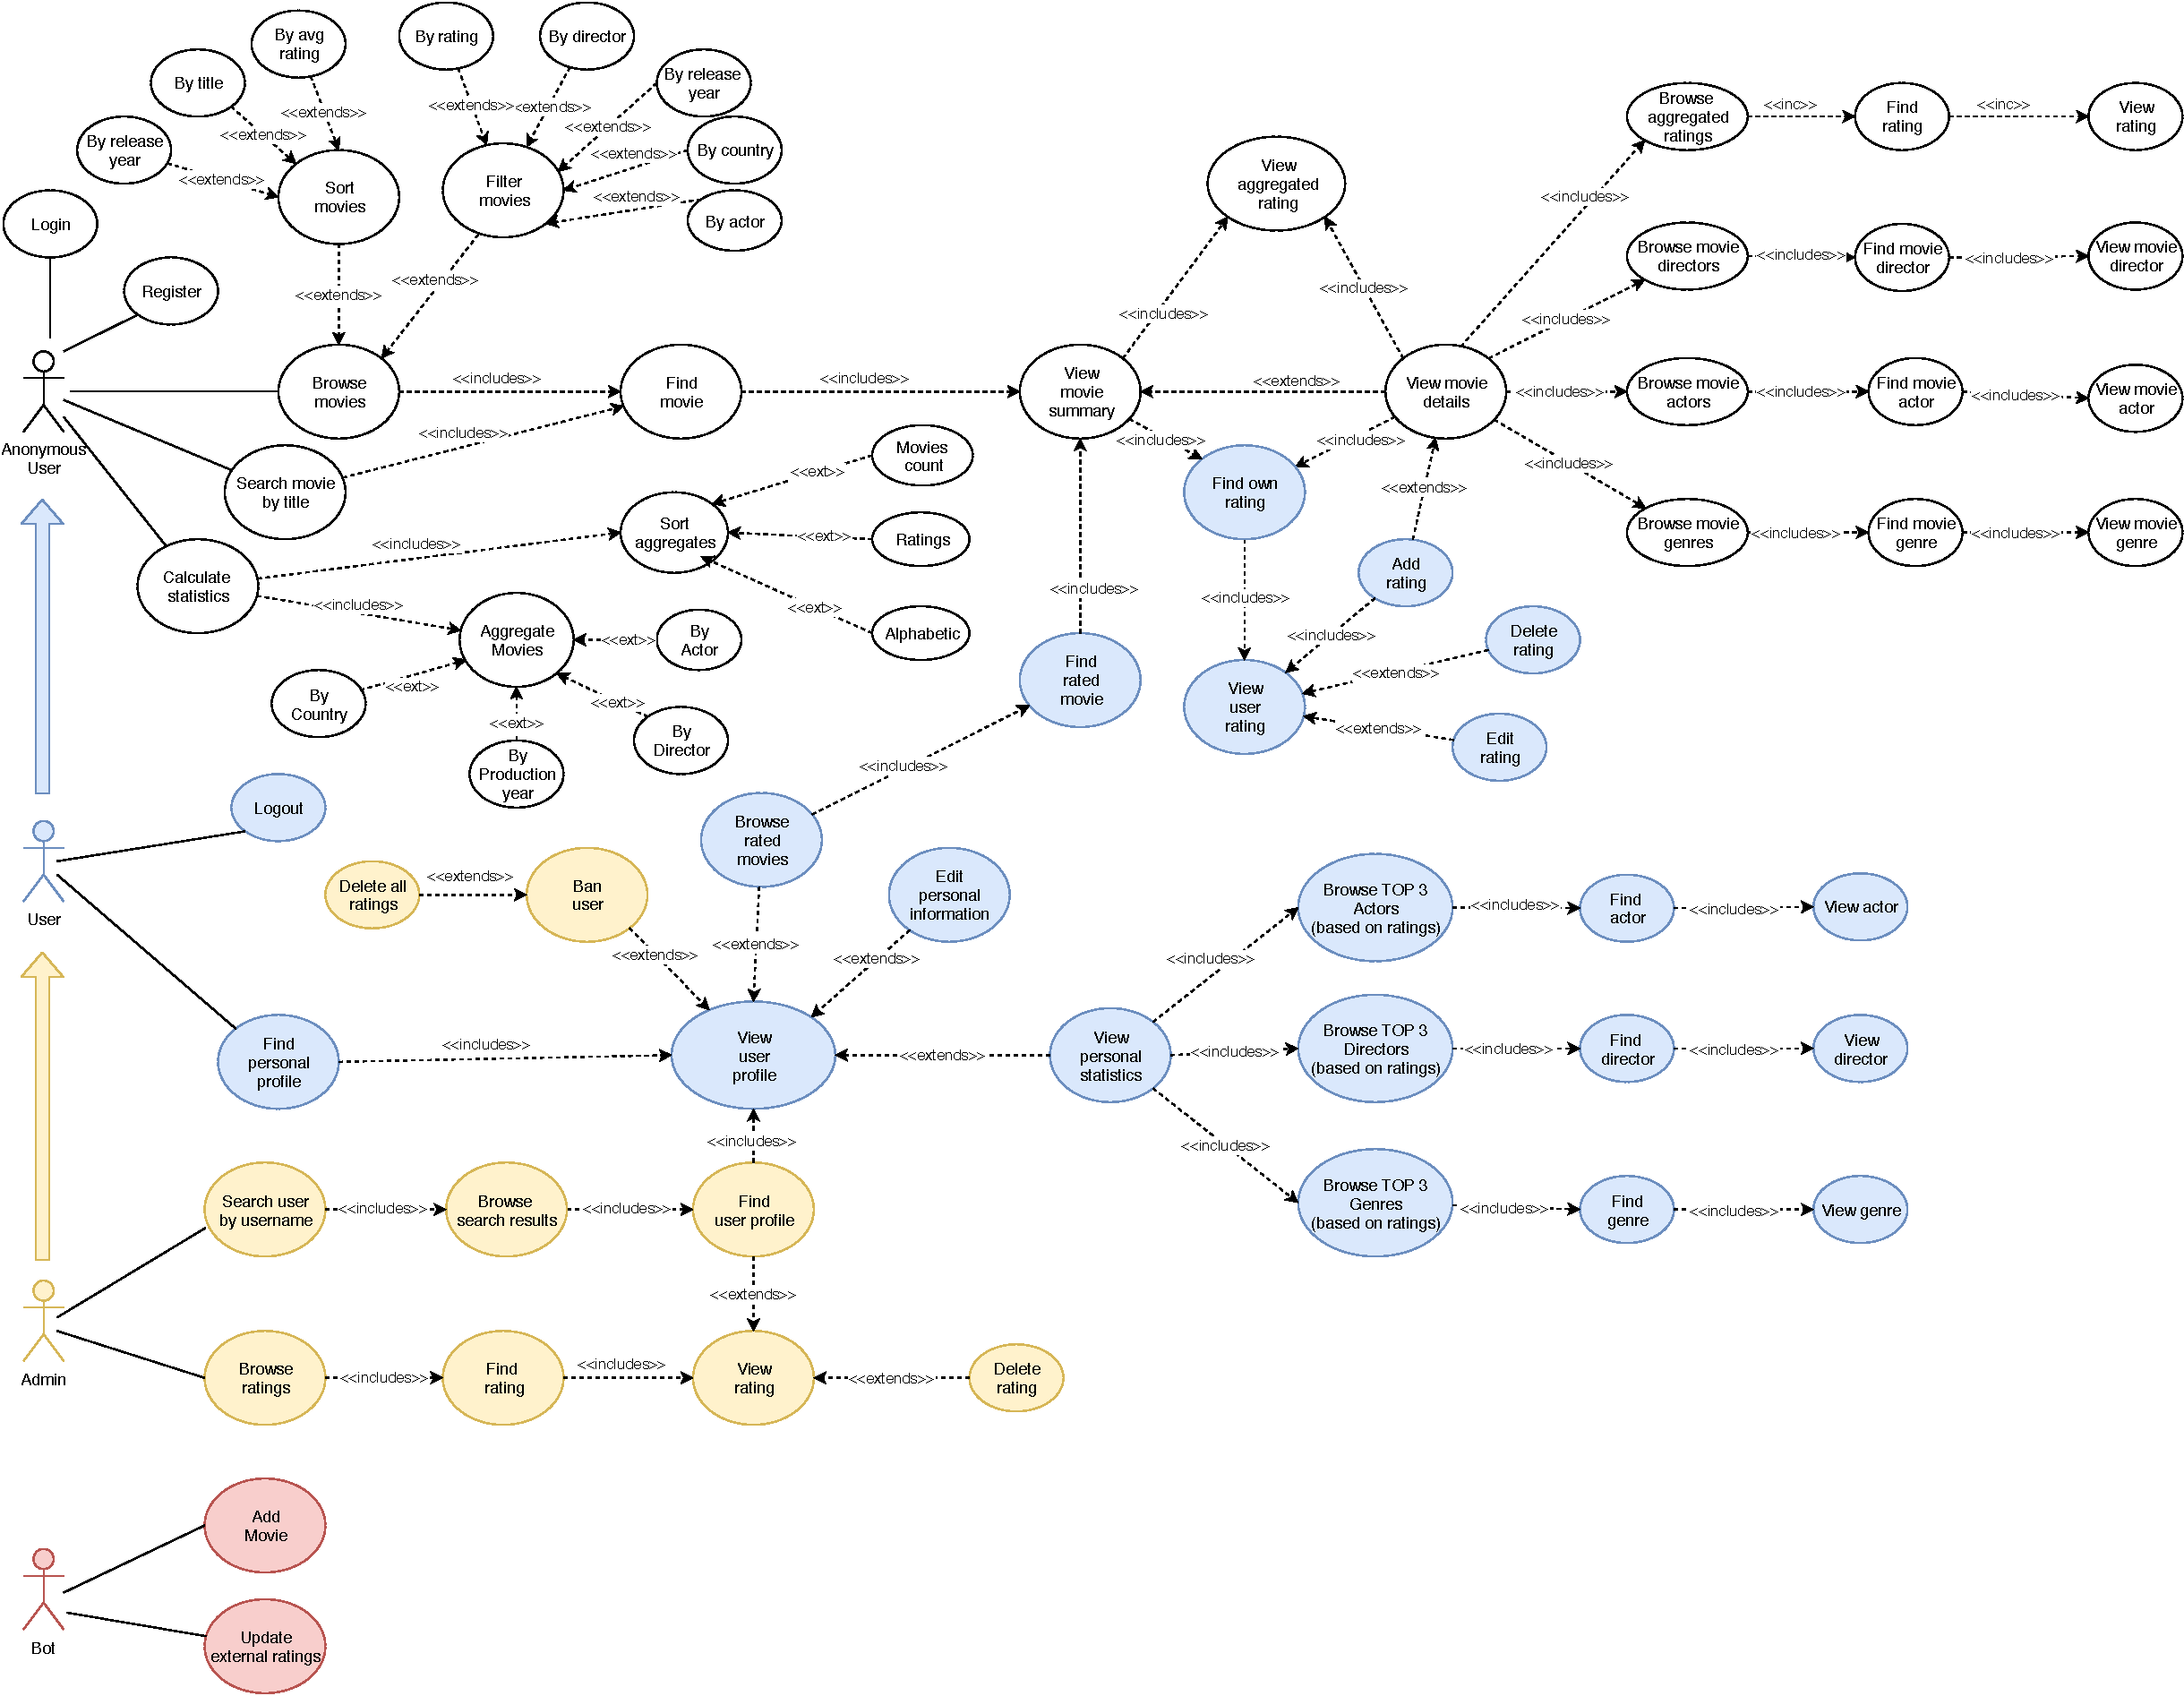
\includegraphics[height=18cm]{figs/use_case.pdf}
    \caption{Use-case diagram}
    \label{fig:usecase}
\end{sidewaysfigure}

The use-case diagram is shown in \cref{fig:usecase}. Different colors are used to highlight cases that are exclusive of some actors: white cases are referred to all users; blue and green cases are referred to registered user and admin; yellow cases are exclusive of the admin. Green cases highlight the ones that 
were introduced in task 3 and all refer to actions that a registered user can
do.

\subsection{Class diagram}

\begin{figure}[h!]
    \centering
    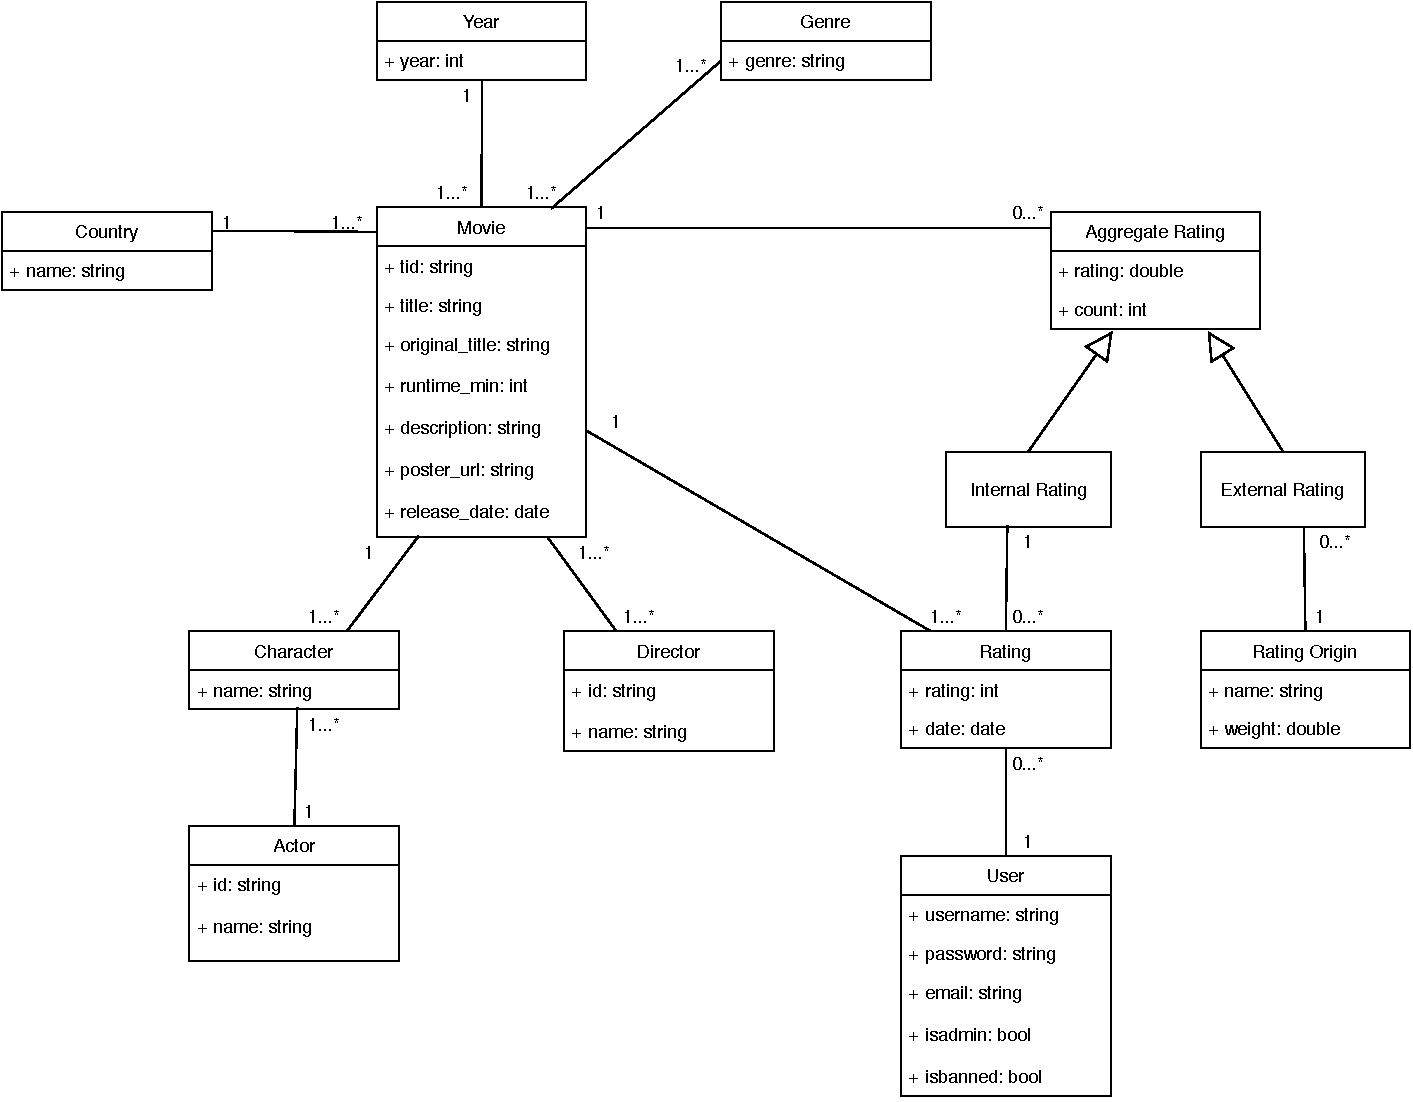
\includegraphics[width=\textwidth]{figs/class_diagram.pdf}
    \caption{Class diagram for the identified entities}
    \label{fig:class_diagram}
\end{figure}

The class diagram is shown in \cref{fig:class_diagram}. It was decided to show \emph{Country}, \emph{Year} and \emph{Genre} as separate entities as they are some of the fields over which aggregate statistics are calculated.

% ------------------------------------------------------------------------------

\clearpage
\subsection{Data model}
\begin{figure}[h!]
    \centering
    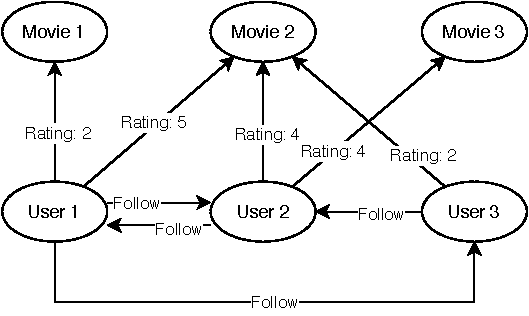
\includegraphics[width=.7\textwidth]{figs/graph_example.pdf}
    \caption{Example graph}
    \label{fig:graph_example}
\end{figure}
The graph database will have 2 different types of nodes and 2 types of edges:
\paragraph{Node types}
\begin{itemize}
	\item \textbf{Movie}: it will contain all information needed to show a list
		of suggested movies: \emph{id}, \emph{title}, \emph{year}, 
        \emph{poster}. In order to efficiently find a movie, an index is added
        to the \emph{id} attribute.
    \item \textbf{User}: it will contain only the \emph{username} and the \emph{\_id} since no other information is required. In order to efficiently find a user, an index is added to both the \emph{id} and the \emph{username}
    attributes (depending on the API, a user can be fetched either by one or 
    the other).
\end{itemize}
\paragraph{Edge types}
\begin{itemize}
	\item \textbf{Rating} (User->Movie): it will contain the \emph{rating} as 
		attribute.
	\item \textbf{Follow} (User->User): no attribute is required.
\end{itemize}
In each following subsection, an example document is shown for every collection.

\subsection{Graph-centric operations}
This section will explain how we intend to execute the queries in the database in terms of graph operations. Simple CRUD operations will not be reported for brevity's sake.

\paragraph{Movie suggestion}
Movie will be suggested based on the ratings of the users that liked similar 
movies as the user we are suggesting to. We consider as liked movies, the ones the user has given a rating greater or equal to 3. For example, in figure \ref{fig:graph_example}, 
\emph{Movie 3} may be suggested to \emph{User 1} since \emph{User 2} liked 
\emph{Movie 2} as \emph{User 1} and he also liked \emph{Movie 3}. 
In practice, starting from a user we will go to each movie he
liked, then to the users who recently liked that movie, then to other movies 
they liked. We will then count the number of paths like the one described 
for each movie (the last one in the path) and show the user the top-N movies 
given this metric.

\paragraph{User suggestion}
Users to follow will be suggested based on the number of common follow 
relationships. For example, in figure \ref{fig:graph_example}, \emph{User 3}
may be suggested to \emph{User 2} since \emph{User 2} follows \emph{User 1}
that follows \emph{User 3}. In practice, starting from the user, we will go to
each user he follows and from here to each user that the latter user follows. 
We will then count the number of paths from the user to the users with common 
followers and show the user the top-N users given this metric.

\subsection{Software Architecture}

The application will be made of the following 4 components:
\begin{itemize}
	\item \textbf{Mongo DB}: a MongoDB cluster will be deployed with
		replication.
	\item \textbf{Neo4j}: an auxiliary graph database will be used to 	
		calculate more efficiently the movie suggestions and to store 
        information about follow relationships since this kind of operations
        are more suited to this kind of DB.
	\item \textbf{React Front-end}: web-based UI.
	\item \textbf{Java Back-end}: using \emph{Spring}, the \emph{Java back-end} will provide REST APIs to the \emph{React front-end}.
	\item \textbf{Updater ``bot''}: three Python scripts are needed in order to nightly update the DB with the latest movies and ratings: 
	\begin{enumerate}
		\item the \textbf{IMDB parser} periodically parses the IMDb dataset to add the latest movies.
		\item the \textbf{scraper} continuously parses the rating sources to update the ratings.
		\item the \textbf{synchronizer} periodically synchronizes movies from MongoDB to Neo4j.
	\end{enumerate}
	These scripts will executes asynchronously from the \emph{Java back-end}.
\end{itemize}

\section{Implementation}

\subsection{Neo4j database}

\subsubsection{Coexistence of two databases}

Providing strict consistency between the two databases is both very complicated
and unnecessary given the application non-functional requirements. Therefore 
we took the path of eventual consistency. Writes that 
involve replicating data on both databases are first stored to MongoDB and then 
asynchronously to Neo4j to reduce perceived latency by the user. 
In case of Neo4j failure, it will be necessary to recover the synchronization 
of the two databases using the script described below. 
This script will be also be executed periodically to update movie details 
(which are updated asynchronously by the scraper scripts and for which we can 
afford a non perfect consistency) and after the IMDB parser script to add 
possible new movies. 

Furthermore, Neo4j contains enough data to prevent a double access to both 
MongoDB and Neo4j in the same user query. However, due to the stricter 
consistency model, authentication is always performed on MongoDB. Therefore some
queries will first need to authenticate using the session id with MongoDB 
before accessing the data stored in Neo4j.

\subsubsection{Database Synchronization}

The Neo4j database will be periodically synchronized by a python script that takes data directly from the document database: useful data is first withdrawn from MongoDB, then they it is post-processed in order to filter out unnecessary attributes before merging into Neo4j. This is done in a Python script using the \textit{pymongo} and \textit{py2neo} modules.

The script manage the synchronization of 3 out of the 4 elements present in our graph database:

\begin{itemize}
	\item \textbf{Movie} nodes;
	\item \textbf{User} nodes;
	\item \textbf{Rated} edge.
\end{itemize}

\textbf{Follows} edges are not managed by the script because they only exists in the graph database.

The work is done by 3 functions (one for each managed element) that simply scan the array of documents that they receives as input in order to keep only the attributes we are interested in. Then they create the relative node and finally they merge it with the current Neo4j database. 

The sync function for the \textbf{Movie} vertex in shown below:
\lstinputlisting[language=Python, firstline=1, lastline=6]{figs/code/consistency.py}

The sync function for the \textbf{User} vertex in shown below:
\lstinputlisting[language=Python, firstline=8, lastline=14]{figs/code/consistency.py}

The sync function for the \textbf{Rating} edge in shown below:
\lstinputlisting[language=Python, firstline=16, lastline=23]{figs/code/consistency.py}

\subsection{Java backend}
\begin{figure}[]
    \centering
    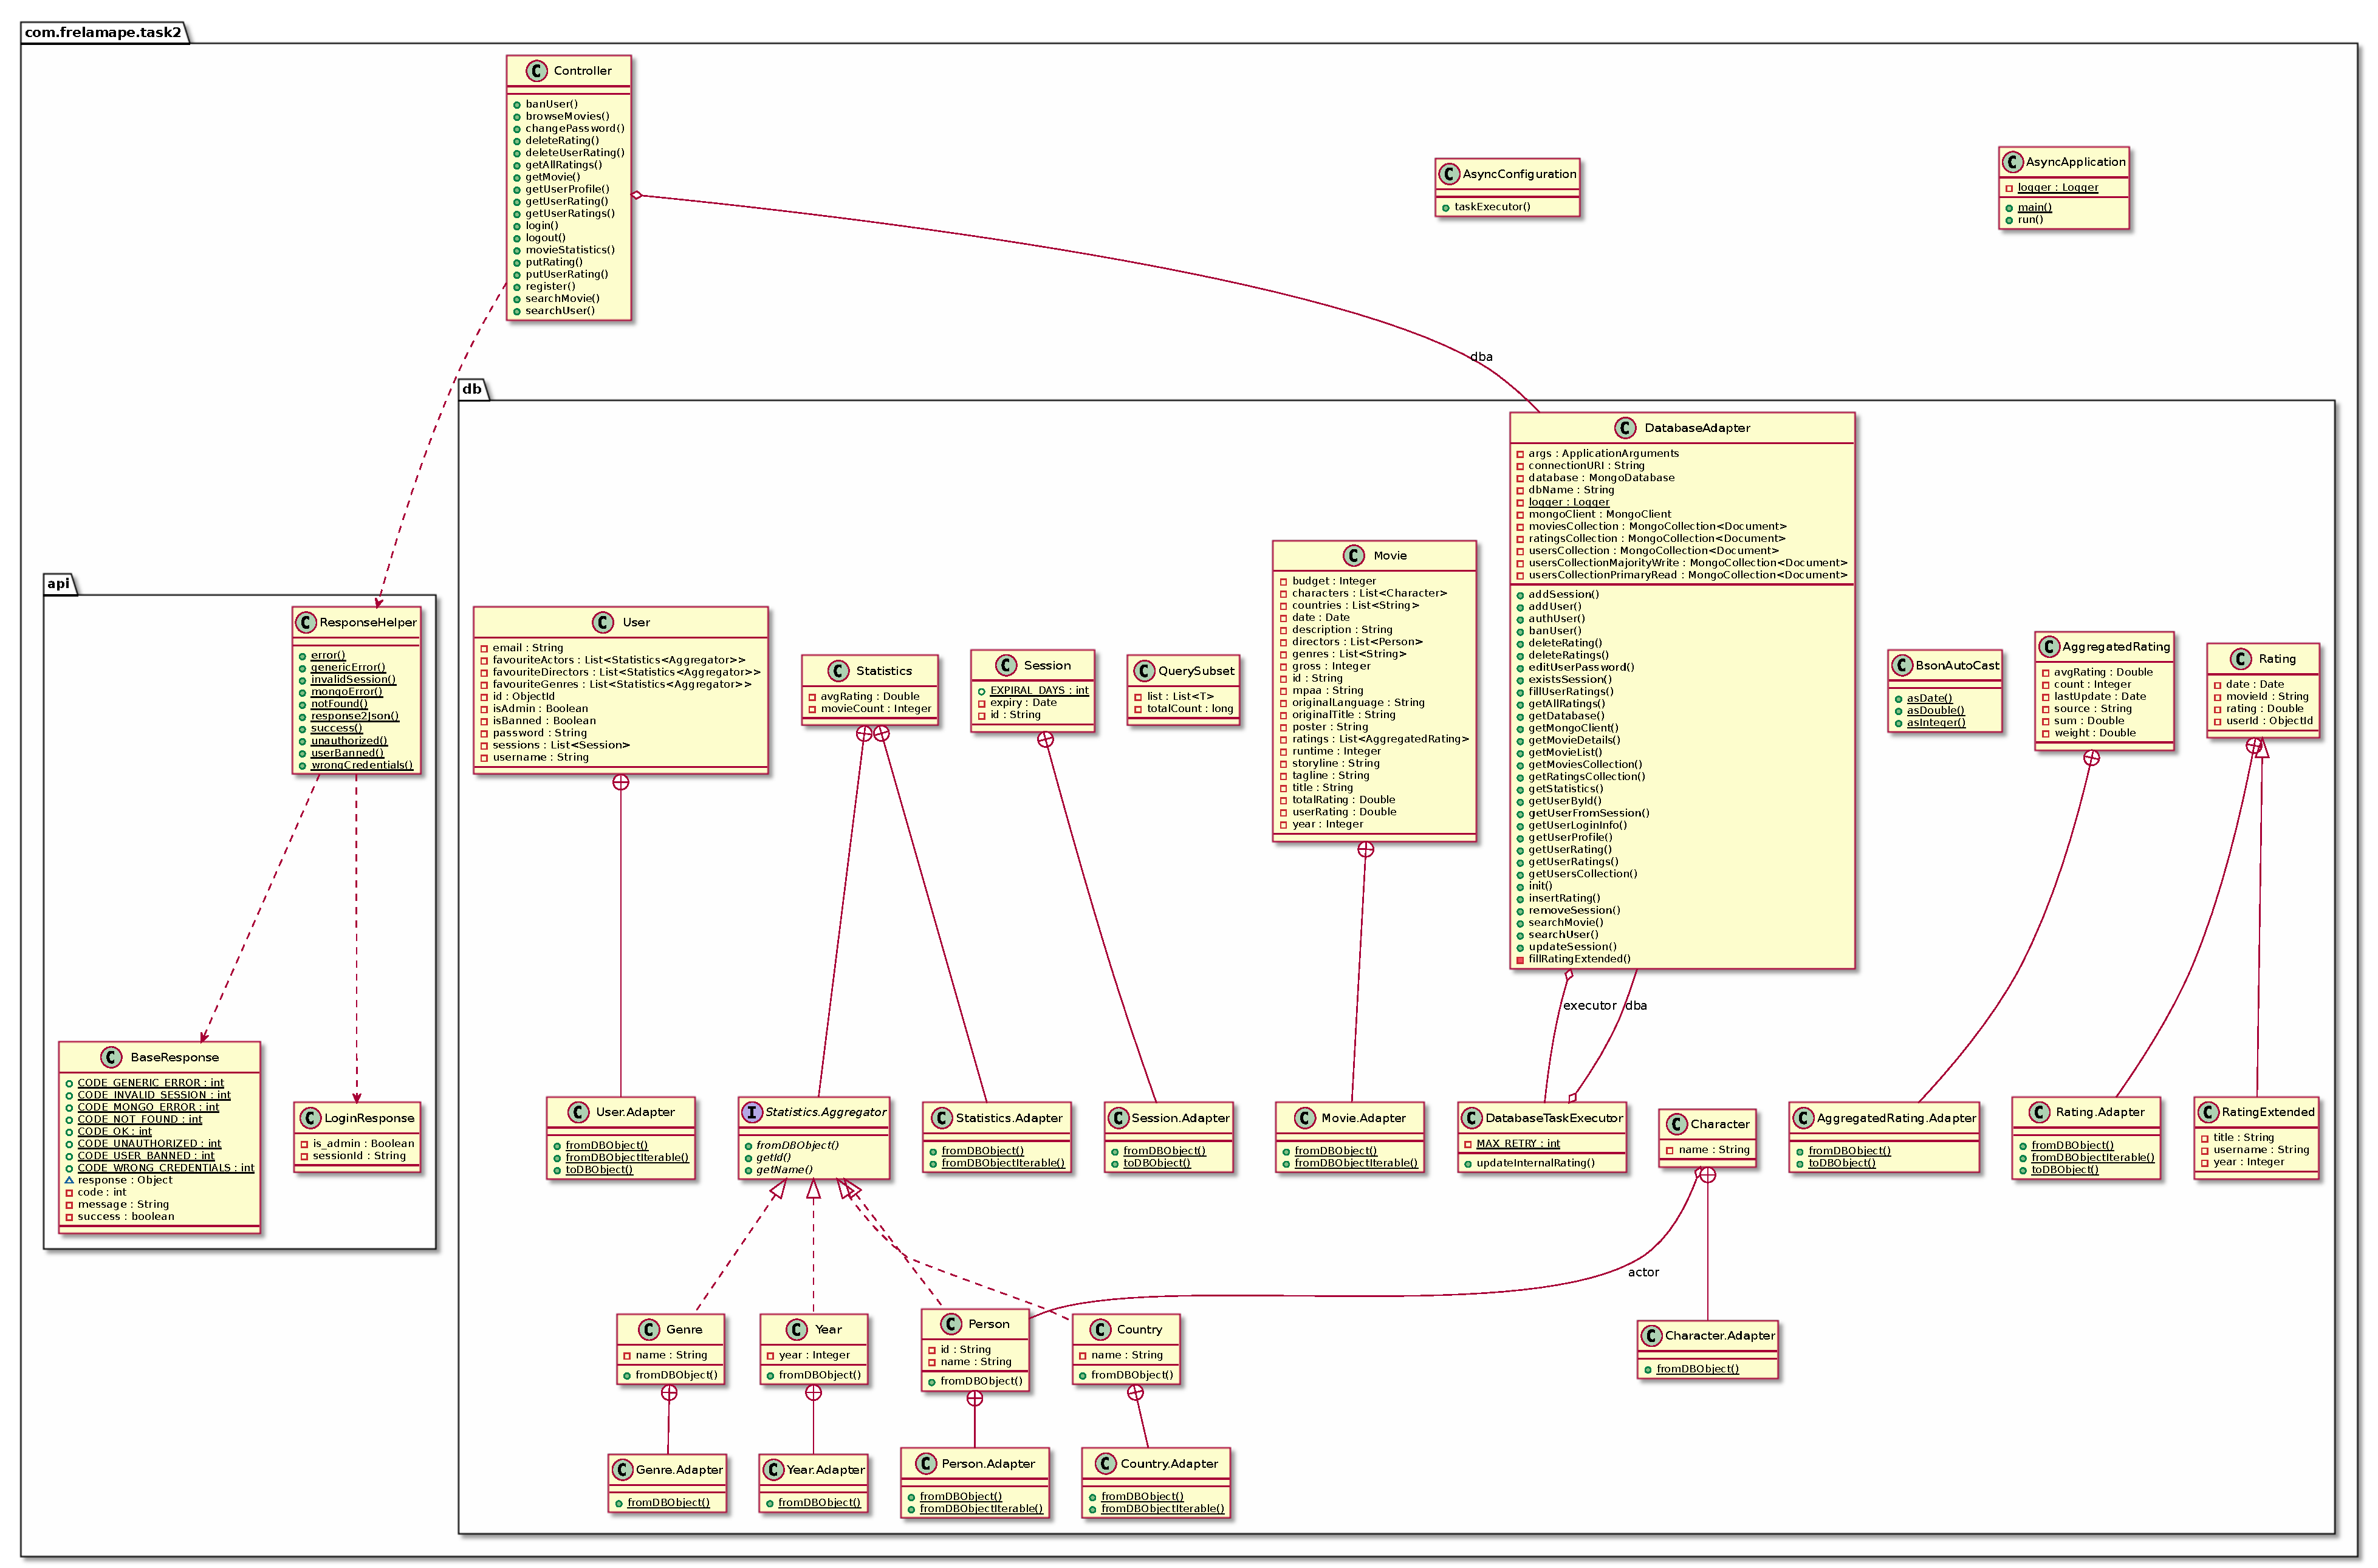
\includegraphics[width=\textheight,angle=90]{figs/backend.pdf}
    \caption{Bird's eye view over the main components of the Java backend.}
    \label{fig:uml-backend}
\end{figure}
\begin{figure}[]
    \centering
    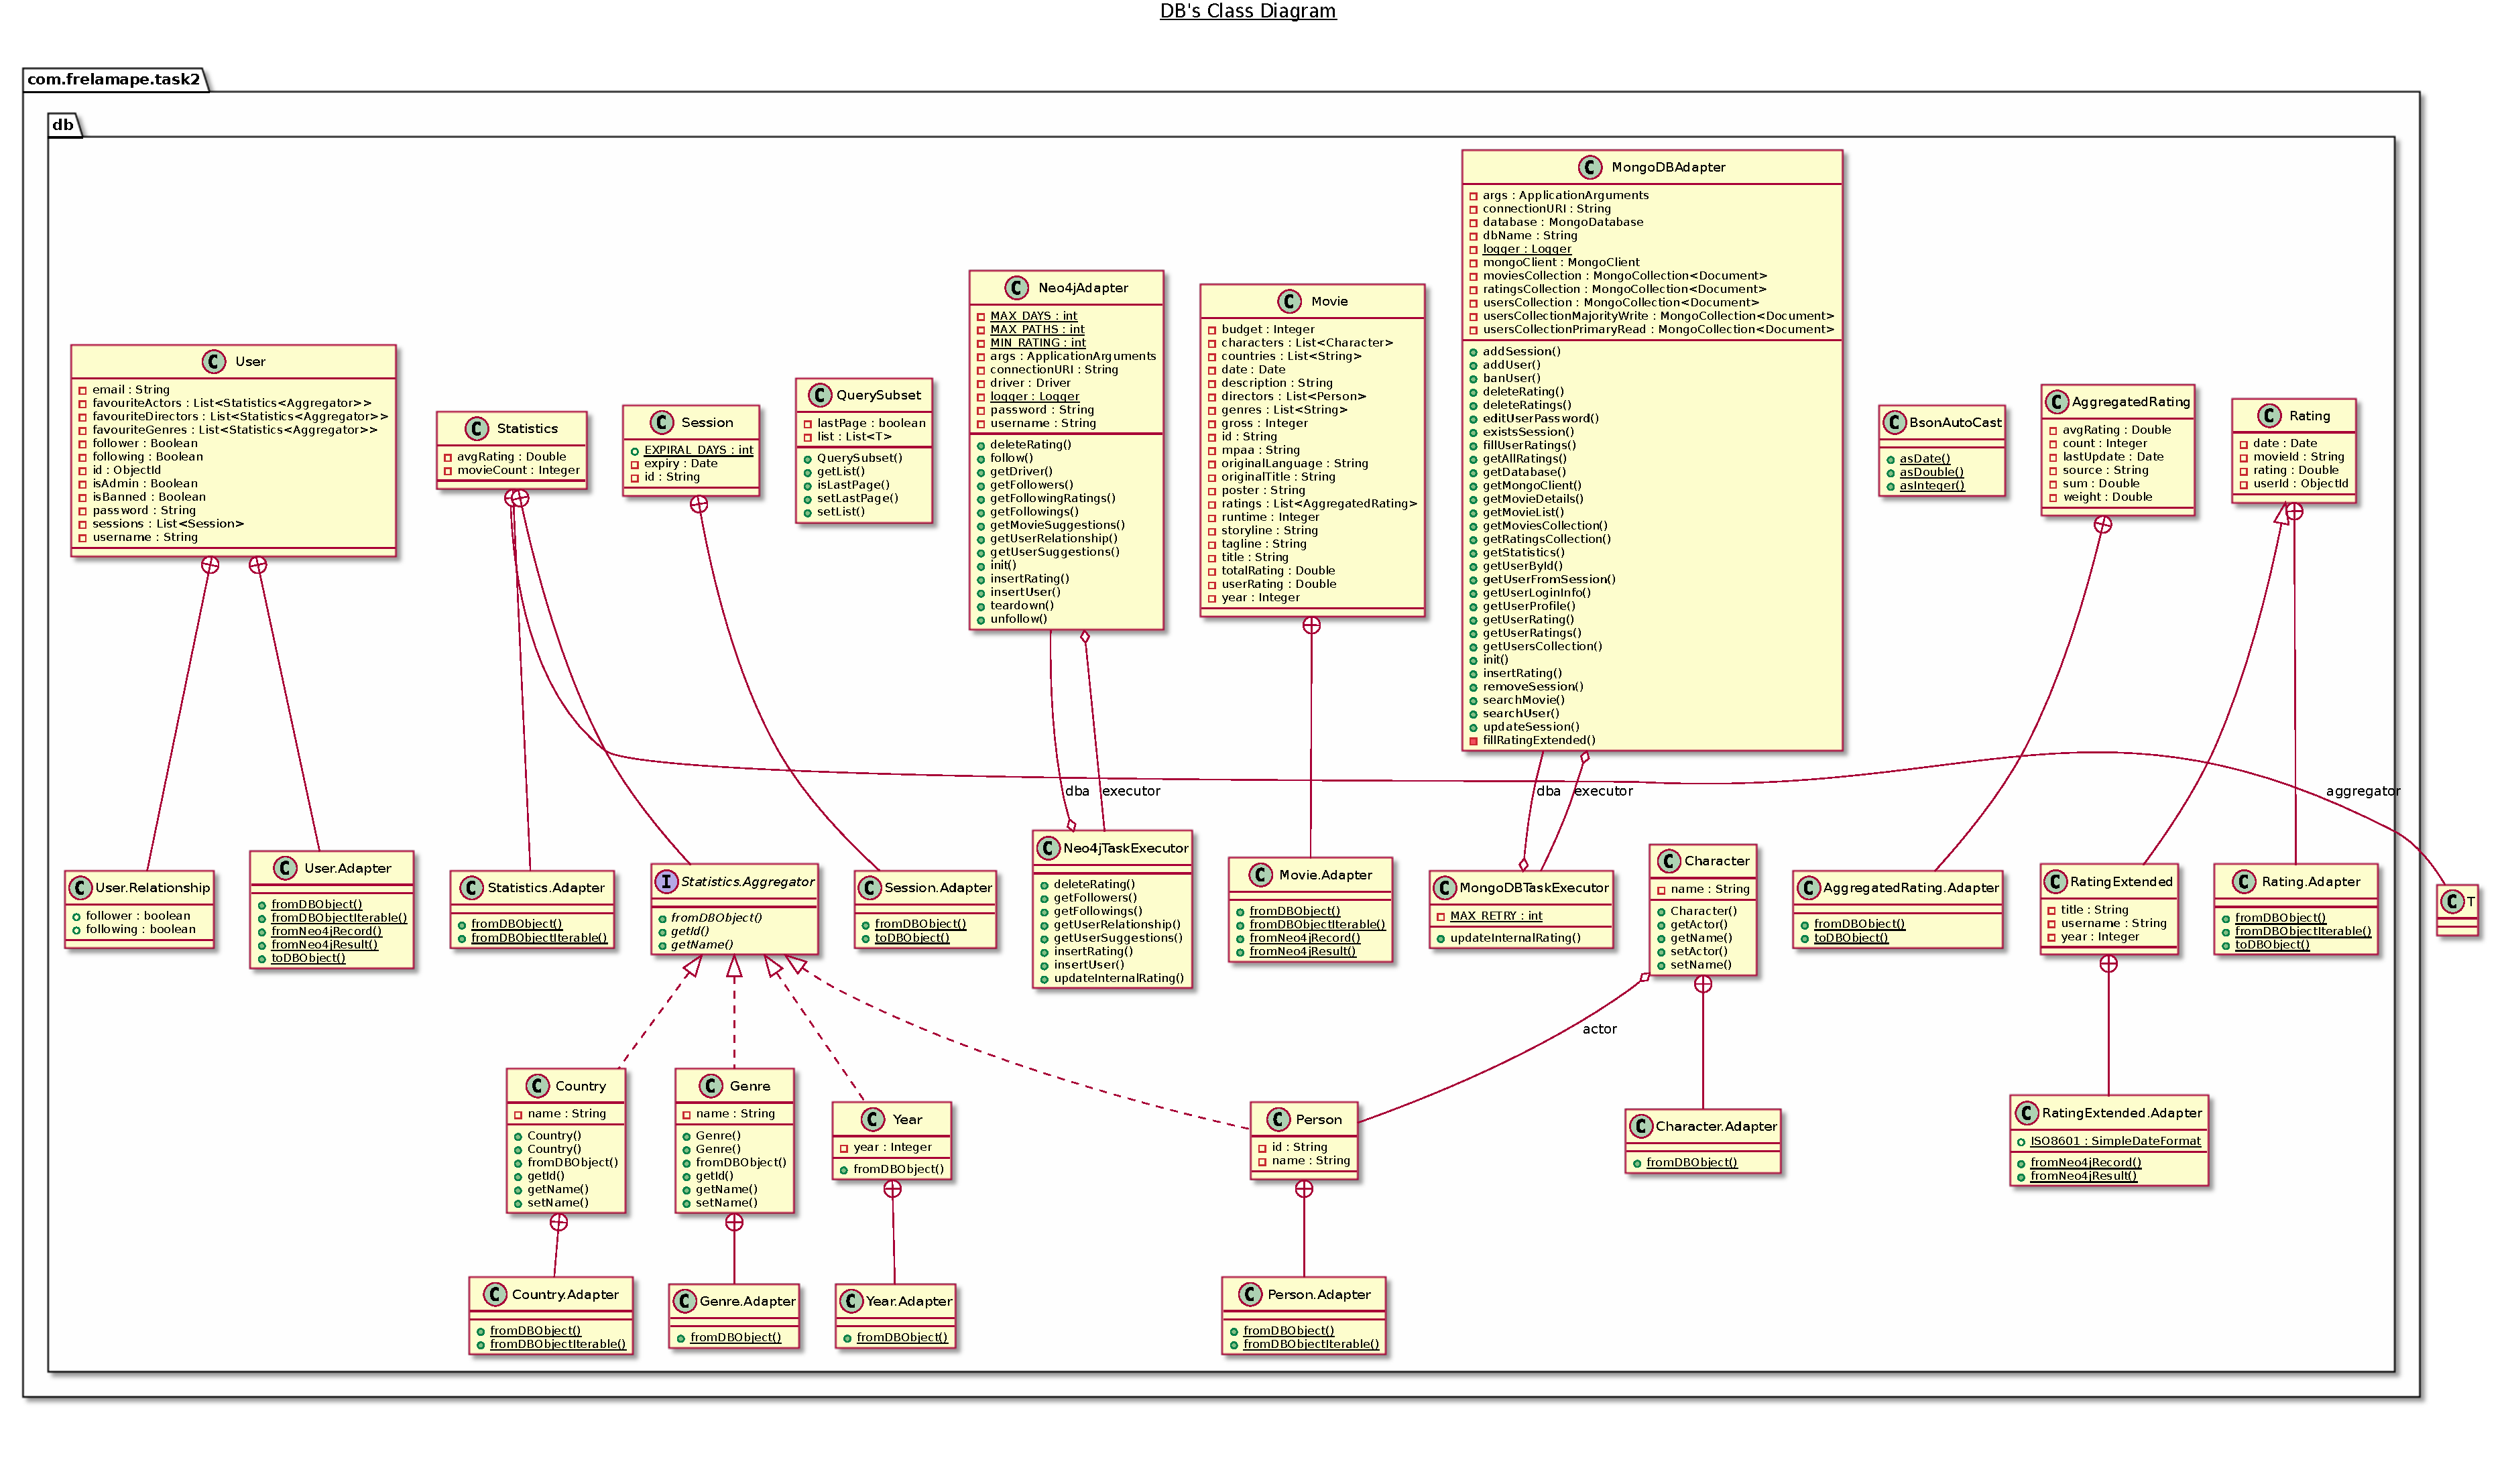
\includegraphics[width=\textheight,angle=90]{figs/db.pdf}
    \caption{Detailed view over the db component of the Java backend.}
    \label{fig:uml-db}
\end{figure}

In figures \ref{fig:uml-backend} and \ref{fig:uml-db} you can see the UML class
diagrams of the Java back-end. The structure is the same as the one presented 
in task 2 with the addition of the \emph{Neo4jAdapter} class which implements the Cypher queries to the Neo4j database (explained in the following sub-section) and of the \emph{Neo4jTaskExecutor} which provides a simple way to asynchronously executing the queries when needed. 


\subsection{Neo4j Queries}
In this section we'll go into details of the queries defined for our Neo4j graph database, according to Cypher query language. Cypher allows users to store and retrieve data from the graph database; its syntax provides a ``visual'' and logical way to match patterns of nodes and relationships in the graph. It is a declarative, SQL-inspired language for describing visual patterns in graphs using ASCII-Art syntax.


\subsubsection{Movie suggestion}
Aim of this query is to return a list of $n$ suggested movies (exploiting \emph{result} object), given as input:
\begin{itemize}
    \item \emph{User u}, the recipient of the suggestions, represented by \emph{\$username} in the query string (according to Cypher syntax);
    \item \emph{int n}, the number of suggestions, represented by \emph{\$limit} in the query string.
\end{itemize}

Earlier we defined what we meant with movie suggestion. However, it is clear that the algorithm provided is inefficient in the sense that it needs to explore a large number of paths. Assuming each user rates in average 50 movies and that a movie has in average 1000 ratings, there are 50*1000*50 = 250000 paths! This is not affordable in such a frequent query. Therefore we need a way to prevent this explosion in the number of paths. The solution we used is 1) to filter out old ratings and -- 2) if this is not sufficient, put a hard limit in the total amount of paths that will be considered in the final aggregation. The first limitation has also a positive side-effect: by keeping only most recent ratings, the most trending movies will be returned to the user. Furthermore, to avoid suggesting always the same movies to the user, for each movie we multiply the score by a random quantity so that the final value is randomly picked from a uniform distribution [score/2; score].

In order to do this filtering, we needed to introduce a Cypher sub-query since \emph{LIMIT} statements can only be placed after a RETURN statement. Please note that the \emph{LIMIT} statement effectively prevents the graph traversal to visit more nodes than necessary.

\lstinputlisting[language=Java, firstline=76, lastline=102, firstnumber=76]{figs/code/Neo4jAdapter.java}

At line 81, starting from the user passed as argument (\emph{u}), we match the movies \emph{m2} as the movies that have been rated by \emph{u2} users, namely the users who share interest (i.e. at least a common liked movie) with \emph{u}. 
From line 82 to line 85 are expressed some meaningful conditions: we only consider \emph{RATED} edges with a rating value higher than \emph{MIN\_RATING}, both for \emph{rum1} and \emph{ru2m1}. This condition ensures that the movie is indeed a common interests among the two users. We also have the condition \emph{ru2m2.rating >= MIN\_RATING} to match only appreciated movies. Another relevant condition is expressed at lines 82-83 using the temporal function \emph{duration.between(..).days < MAX\_DAYS}, whose scope is to filter rating edges, considering only movies rated during the last week.

\subsubsection{User suggestion}
Aim of this query is to return the relationships between user 1 and user 2, exploiting a \emph{User.Relationship} instance that indicates whether user 1 follows user 2 (following) and whether user 2 follows user 1 (followed).
\emph{getUserRelationship} method takes 2 arguments:

\begin{itemize}
    \item \emph{u1}, first user, whose username becomes \emph{\$username1} query parameter;
    \item \emph{u2}, second user, whose username becomes \emph{\$username2} query parameter.
\end{itemize}

The same problem of ``number of paths explosion'' that we seen could happen also in this query. Therefore the same approach as before (without the temporal limitation). We also applied the same randomization technique as before.

\lstinputlisting[language=Java, firstline=115, lastline=134, firstnumber=115]{figs/code/Neo4jAdapter.java}

At lines 118-119 the addressed user vertices are matched by username parameter and referred by \emph{u1} and \emph{u2}.
At lines 120-121 we use a predicate function \emph{EXISTS()}, whose scope is to return true if exists an edge between \emph{u1} and \emph{u2} and the other way around.
Each Cypher execution returns a stream of records, each record has two properties that represent the boolean flag for the presence or not of relationship between the 2 user nodes.
\subsubsection{Other queries}

\paragraph{User creation} Creates a new user.

\begin{lstlisting}[language=Cypher]
CREATE (:User {_id: $id, username: $username})
\end{lstlisting}

\paragraph{Rating insertion/update} This operations creates a new rating, if none already exists, otherwise updates the rating already in the DB.

\begin{lstlisting}[language=Cypher]
MATCH (m:Movie {_id: $movie_id})
MATCH (u:User {_id: $user_id})
MERGE (u)-[r:RATED]->(m)
SET r.rating=$rating, r.date=$date
\end{lstlisting}

\paragraph{Rating deletion} Removes a rating.

\begin{lstlisting}[language=Cypher]
MATCH (m:Movie {_id: $movie_id})
MATCH (u:User {_id: $user_id})
MATCH (u)-[r:RATED]->(m)
DELETE r
\end{lstlisting}

\paragraph{Follow user} A started following B.

\begin{lstlisting}[language=Cypher]
MATCH (a:User {username: $username_a})
MATCH (b:User {username: $username_b})
MERGE (a)-[:FOLLOWS]->(b)
\end{lstlisting}

\paragraph{Un-follow user} A stopped following B.

\begin{lstlisting}[language=Cypher]
MATCH (a:User {username: $username_a})
MATCH (b:User {username: $username_b})
MATCH (a)-[r:FOLLOWS]->(b)
DELETE r
\end{lstlisting}

\paragraph{Ratings of followed users} Returns a (paged) list of all ratings by followed users in chronological order (most recent first). \emph{skip} and \emph{limit} are set so that only the requested page of $n$ elements is returned.

\begin{lstlisting}[language=Cypher]
MATCH (:User {username: $username})-[:FOLLOWS]->(u:User)-[r:RATED]->(m:Movie)RETURN r.date as date, r.rating as rating,
    m._id as movie_id, m.title as title, m.year as year, m.poster as poster,
    u._id as user_id, u.username as username
ORDER BY r.date DESC
SKIP $skip
LIMIT $limit
\end{lstlisting}

\paragraph{List of Followed Users} Returns the list of the users that a given user (\emph{me} in the query) is following. Furthermore, the query returns the relationship between the returned \emph{user} and a third user (called \emph{pov} in the query), i.e. whether \emph{pow} is \emph{following} \emph{user} and whether \emph{user} is a follower of \emph{pov}. 

\begin{lstlisting}[language=Cypher]
MATCH (me:User {username: $username})
MATCH (me)-[:FOLLOWS]->(user:User)
MATCH (pov:User {username: $username_pov})
RETURN user.username as username, user._id as _id,
    EXISTS((pov)-[:FOLLOWS]->(user)) as following,
    EXISTS((user)-[:FOLLOWS]->(pov)) as follower
ORDER BY user.username "
SKIP $skip
LIMIT $limit
\end{lstlisting}

\paragraph{List of Followers} Returns the list of the users that follow a given user (\emph{me} in the query). Furthermore, the query returns the relationship between the returned \emph{user} and a third user (called \emph{pov} in the query), i.e. whether \emph{pow} is \emph{following} \emph{user} and whether \emph{user} is a follower of \emph{pov}. 

\begin{lstlisting}[language=Cypher]
MATCH (me:User {username: $username})
MATCH (user)-[:FOLLOWS]->(me:User)
MATCH (pov:User {username: $username_pov})
RETURN user.username as username, user._id as _id,
    EXISTS((pov)-[:FOLLOWS]->(user)) as following,
    EXISTS((user)-[:FOLLOWS]->(pov)) as follower
ORDER BY user.username "
SKIP $skip
LIMIT $limit
\end{lstlisting}

\paragraph{Users relationship} Returns the relationship between user 1 and user 2, i.e. whether \emph{u1} is \emph{following} B and whether A is a follower of \emph{u2}. 

\begin{lstlisting}[language=Cypher]
MATCH (u1:User {username: $username1})
MATCH (u2:User {username: $username2})
RETURN EXISTS((u1)-[:FOLLOWS]->(u2)),
    EXISTS((u2)-[:FOLLOWS]->(u1))
\end{lstlisting}

\section{Tests}
This section reports some tests that have been performed in order to evaluate 
the performance of the Neo4j database.

Before running the tests, random users, ratings and follow relationships have 
been created. In particular, 100 test users have been created and, for each 
user, 50 ratings and 10 follow relationships to another user. In order to 
better test the movie suggestion functionality, the ratings have been restricted
to a subset of 1000 movies (instead of the full $\sim50k$ movies).

In each of the following experiments, each data point has been obtained running 
the \emph{siege} application with 100 concurrent users and no delay between 
requests for 1 minute on a random subset of the possible queries. Experiments 
have been executed on one of the virtual machines provided by the University 
of Pisa (1 virtual CPU core, 8GB of RAM).

\subsection{Movie suggestion}
As already discussed before, the movie suggestion query cannot afford to look
up all possible paths and for this reason a limit in the maximum number of paths
along which the aggregation is computed has been reduced. This subsection 
shows how we decided to use 100 as limit.

In figure \ref{fig:tps_mp}, we reported the number of handled requests every 
second (i.e. transactions-per-second, tps, in \emph{siege} jargon) for the 
movie suggestion query with different limits on the maximum number of paths to 
take into consideration. From the plot, it can be seen that the throughput 
drastically decreases already in the first step from 100 to 200. For this 
reason, we decided to set it to set it to 100, which provides an acceptable 
throughput (around 450). Of course this reasoning holds only for the current 
configuration on the VM provided by the University of Pisa.

In order to further increase the throughput of this very frequent query, the 
introduction of an in-memory database could be taken into consideration. This database could store the suggested movies to the user for as long as the user is active in the website (few minutes) in case the user goes to the homepage again (which is very likely). It is not advisable to cache this value longer since this would make suggestions too static, which we do not want for a better user experience.

\begin{figure}[]
    \centering
    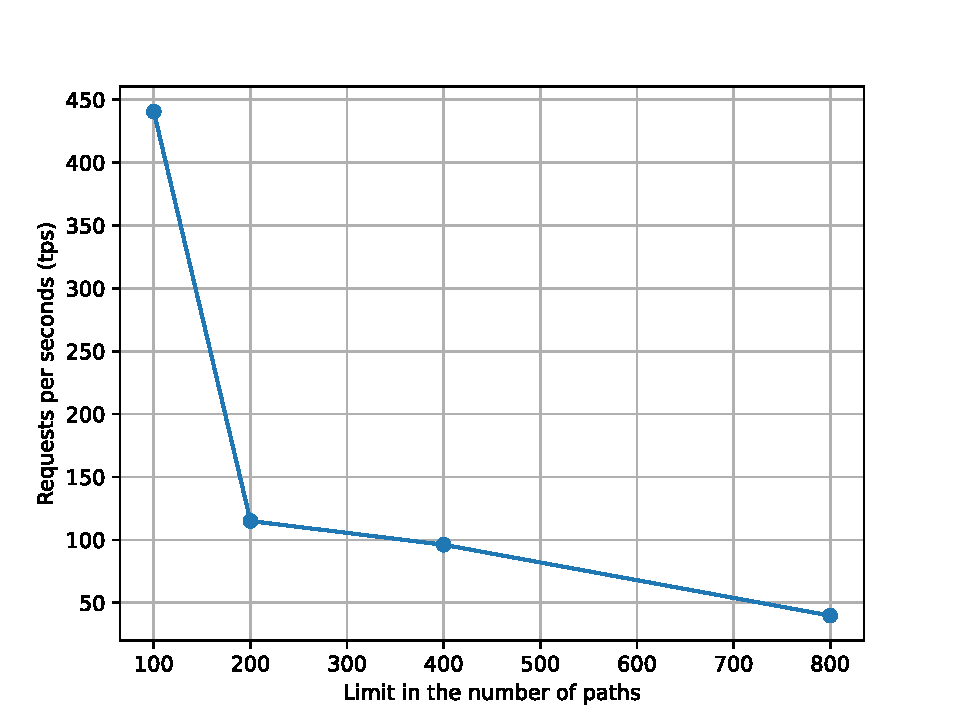
\includegraphics[width=\textwidth]{figs/tps_max_path.pdf}
    \caption{Plot of the handled requests per second for the movie suggestion query at different limits on the maximum number of paths.}
    \label{fig:tps_mp}
\end{figure}

\subsection{Comparison of other common queries}
In this subsection, the throughput of the most common queries on the graph 
database is reported. The queries we took into consideration are:
\begin{itemize}
    \item Ratings of followed users
    \item List of followers/following users
    \item Suggestion of movies
    \item Suggestion of users
\end{itemize}

Other queries, like ratings, users and follow relationships insertion and 
deletion have been ignored in the analysis since they represent just a very 
small amount of the total queries to the back-end.

\begin{figure}[]
    \centering
    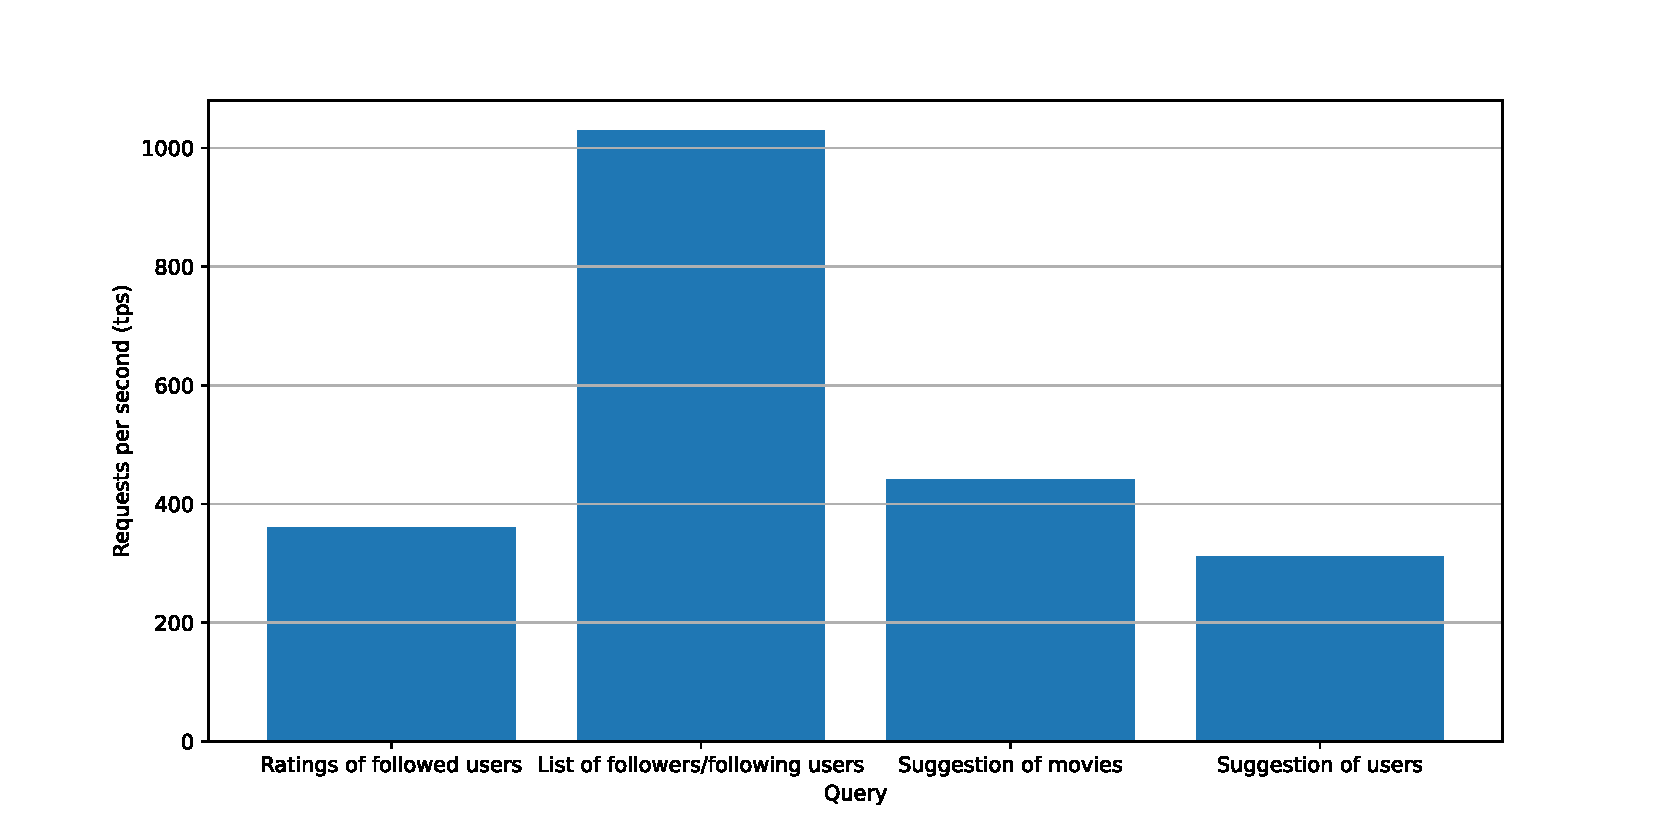
\includegraphics[width=\textwidth]{figs/tps_query.pdf}
    \caption{Bar plot of the throughput of different queries to the graph database}
    \label{fig:queries-graph}
\end{figure}

\begin{figure}[]
    \centering
    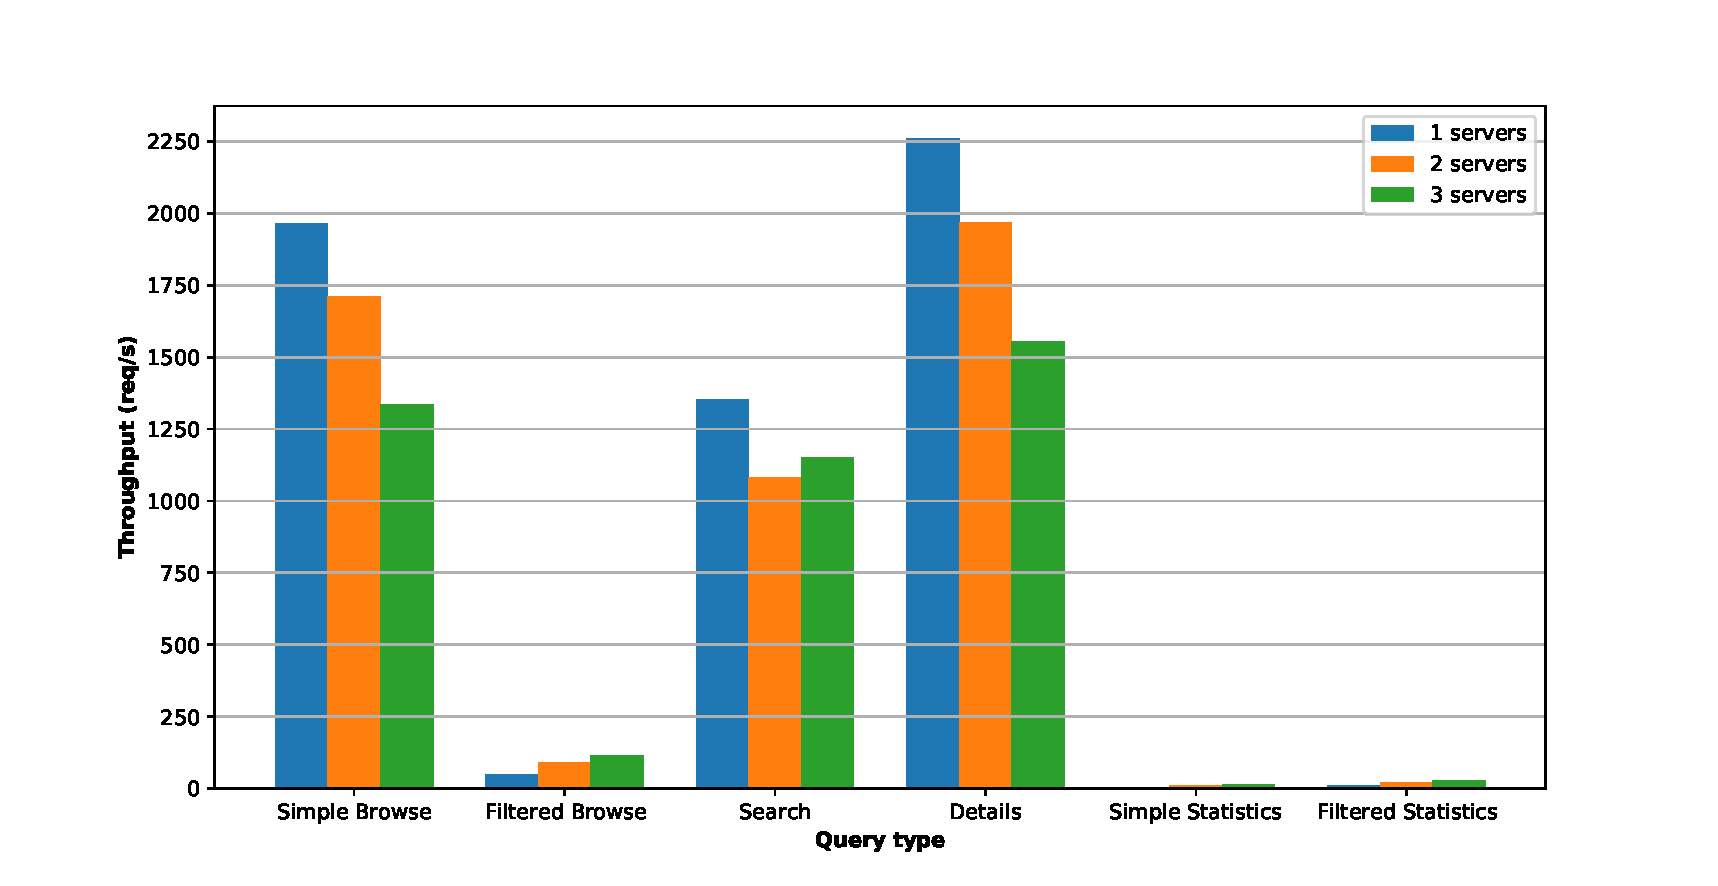
\includegraphics[width=\textwidth]{figs/siege_barplot_all.pdf}
    \caption{Bar plot of the throughput of different queries to the document database}
    \label{fig:queries-mongo}
\end{figure}

In figure \ref{fig:queries-graph} we can see the throughput of queries to Neo4j.
The results obtained for the other queries to MongoDB is also shown as a
reference in figure \ref{fig:queries-mongo}. From the figures we can see how 
Neo4j is significantly slower than MongoDB, if we consider the highest 
performing queries of both. However, it must be noted that the aforementioned
queries on MongoDB are much ``simpler'' than the ones on Neo4j.

Focusing on Neo4j queries, we can note that the fastest is the list of 
followers/following users and this was expected since it's the most simple 
query that just requires to show all adjacent nodes. Next we have the 
other three queries that are all quite close to each other. It may look quite
surprising to see that the suggestion of movies is faster that the list of 
ratings of followed users but there are two things to be taken into 
consideration. First, the suggestion of movies just looks 100 paths (as for 
the previous set of experiments). Second, the ratings of followed users has 
to perform an expensive order by operation before returning the requested page.
In the last place, we can find the suggestion of users, which is slower due to 
the fact that it has to check that returned users are not already followed by 
the user performing the query in a sub-query.

\end{document}
